% !TeX root = ./TMA03.tex
The Lloyd polynomial $L_2(x)$ will be shown to be
\[
	2L_2(x) = 4x^2 - 4(n+1)x + (n^2 + n +2)
\]
as follows.

From \textbf{Theorem~9.6} if there exists a perfect $(n,M,2t+1)$-code over $GF(q)$ then the Lloyd polynomial is given by\marginnote{\hill p103.}[-0.5cm]
\[
	L_t(x) =\sum_{j=0}^t (-1)^j(q-1)^{t-j}\binom{x-1}{j}\binom{n-x}{t-j}
\]
and has $t$ distinct roots in the interval $1\leq x\leq n$.

In our case, $q=2$ and $t=2$ so we have
\[
	L_2(x) =\sum_{j=0}^2 (-1)^j\binom{x-1}{j}\binom{n-x}{2-j},
\]
which becomes
\[
	L_2(x) = \binom{x-1}{0}\binom{n-x}{2} -\binom{x-1}{1}\binom{n-x}{1}+\binom{x-1}{2}\binom{n-x}{0}.
\]
Expanding the binomial coefficients we obtain
\begin{align*}
	L_2(x) &= \frac{(n-x)(n-x-1)}{2} - (x-1)(n-x) + \frac{(x-1)(x-2)}{2}.
\end{align*}
Then,
\begin{align*}
	2L_2(x) &= (n-x)(n-x-1) - 2(x-1)(n-x) + (x-1)(x-2),\\
&= n^2 - 2nx -n + x^2 +x -2\left(nx -x^2 -n +x\right) + x^2 -3x + 2,\\
&= n^2 - 4nx + n + 4x^2 -2x +2,\\
&= 4x^2 -4x(n+1) + (n^2 + n + 2)\text{ as required.}
\end{align*}
\begin{figure}[H]
\centering
  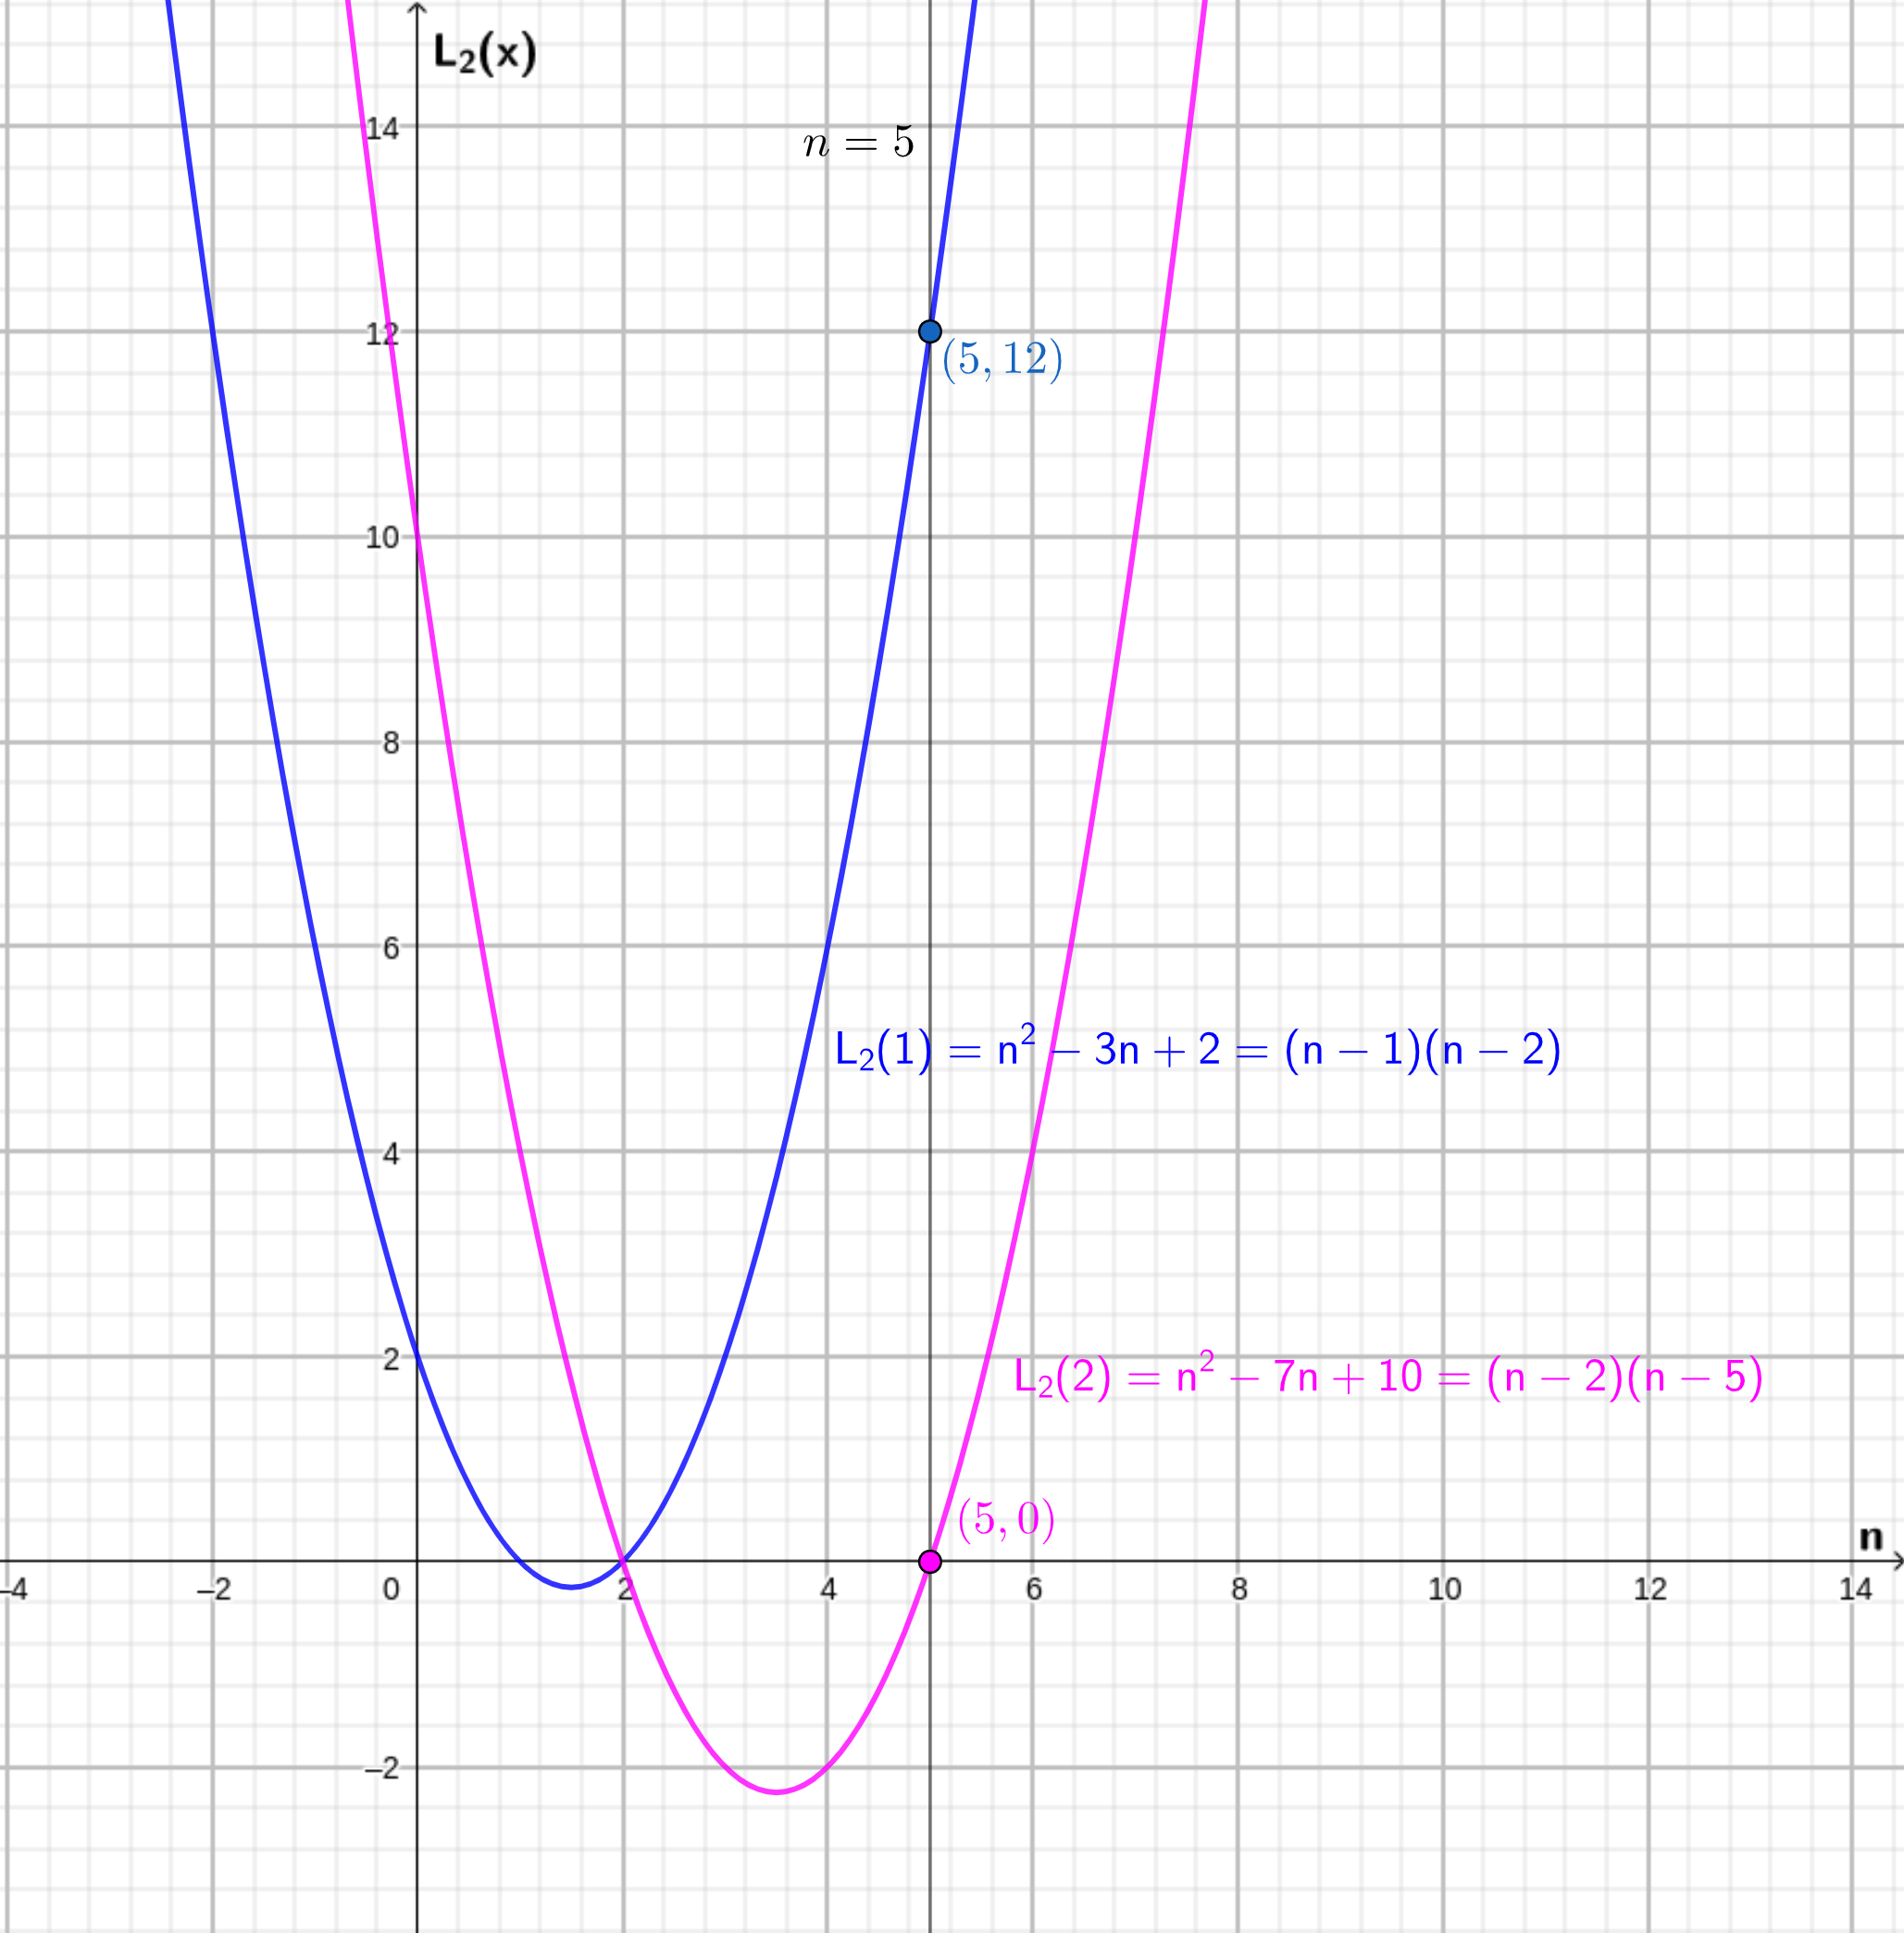
\includegraphics[width=0.8\linewidth]{q2b.png}
  \caption{Plots of $L_2(1)$ and $L_2(2)$ against $n$ showing that when $n>5$ neither $L_2(1)$ nor $L_2(2 )$ is zero.}
  \label{fig:graph1}
\end{figure}
Shown in Figure~\ref{fig:graph1} are plots of $L_2(1)$ and $L_2(2)$ against $n$ which shows for $n=5$ that $L_2(1)=12$ and $L_2(2)=0$. As both plots are quadratic with roots shown, neither plot crosses the $x$-axis again so as $n$ increases beyond $5$ both $L_2(1)$ and $L_2(2)$ also increase. So neither $L_2(1)$ nor $L_2(2)$ is zero for $n>5$.